\documentclass[12pt,a4paper]{article}
\usepackage[utf8]{inputenc}
\usepackage{bold-extra}
\usepackage[pdfauthor={Luciano Henrique de Oliveira Santos}]{hyperref}
\usepackage[right=2.5cm,left=2.5cm,top=2cm,bottom=2cm]{geometry}
\usepackage{url}
\usepackage{graphicx}
\usepackage{float}
\usepackage{setspace}
\usepackage[export]{adjustbox}
\usepackage[usenames,dvipsnames]{xcolor}
\usepackage{listings}
\usepackage{textcomp}


\renewcommand{\familydefault}{\sfdefault}

\title{Clue in Prolog\\{\Large -- A Didactic Example --}}
\author{Luciano Santos}
\date{August 2016}

\newcommand{\varname}[1]{\texttt{#1}}
\newcommand{\varnameit}[1]{\textit{\texttt{#1}}}
\newcommand{\varnamebf}[1]{\textbf{\texttt{#1}}}
\newcommand{\varnamebfit}[1]{\textbf{\textit{\texttt{#1}}}}

\newcommand{\predprot}[2]{{\color{MidnightBlue}\varnamebf{#1}}/{\color{Mulberry}\varname{#2}}}
\newcommand{\predname}[1]{{\color{MidnightBlue}\varname{#1}}}

% --- ugly internals for language definition ---
% see: http://tex.stackexchange.com/questions/161235/can-the-listings-package-be-set-up-to-highlight-prolog-code-like-minted-does
%
\makeatletter

\newcommand\PrologPredicateStyle{}
\newcommand\PrologVarStyle{}
\newcommand\PrologAnonymVarStyle{}
\newcommand\PrologOpStyle{}
\newcommand\PrologAtomStyle{}
\newcommand\PrologOtherStyle{}
\newcommand\PrologCommentStyle{}


% useful switches (to keep track of context)

\newif\ifpredicate@prolog@
\newif\ifwithinparens@prolog@

% save definition of underscore for test
\lst@SaveOutputDef{`_}\underscore@prolog

% local variables
\newcount\currentchar@prolog

\newcommand\@testChar@prolog%
{%
  % if we're in processing mode...
  \ifnum\lst@mode=\lst@Pmode%
    \detectTypeAndHighlight@prolog%
  \else
    % ... or within parentheses
    \ifwithinparens@prolog@%
      \detectTypeAndHighlight@prolog%
    \fi
  \fi
  % Some housekeeping...
  \global\predicate@prolog@false%
}

% helper macros
\newcommand\detectTypeAndHighlight@prolog
{%
  % First, assume that we have an atom.
  \def\lst@thestyle{\PrologAtomStyle}%
  % Test whether we have a predicate and modify the style accordingly.
  \ifpredicate@prolog@%
    \def\lst@thestyle{\PrologPredicateStyle}%
  \else
    % Test whether we have a predicate and modify the style accordingly.
    \expandafter\splitfirstchar@prolog\expandafter{\the\lst@token}%
    % Check whether the identifier starts by an underscore.
    \expandafter\ifx\@testChar@prolog\underscore@prolog%
      % Check whether the identifier is '_' (anonymous variable)
      \ifnum\lst@length=1%
        \let\lst@thestyle\PrologAnonymVarStyle%
      \else
        \let\lst@thestyle\PrologVarStyle%
      \fi
    \else
      % Check whether the identifier starts by a capital letter.
      \currentchar@prolog=65
      \loop
        \expandafter\ifnum\expandafter`\@testChar@prolog=\currentchar@prolog%
          \let\lst@thestyle\PrologVarStyle%
          \let\iterate\relax
        \fi
        \advance \currentchar@prolog by 1
        \unless\ifnum\currentchar@prolog>90
      \repeat
    \fi
  \fi
}
\newcommand\splitfirstchar@prolog{}
\def\splitfirstchar@prolog#1{\@splitfirstchar@prolog#1\relax}
\newcommand\@splitfirstchar@prolog{}
\def\@splitfirstchar@prolog#1#2\relax{\def\@testChar@prolog{#1}}

% helper macro for () delimiters
\def\beginlstdelim#1#2%
{%
  \def\endlstdelim{\PrologOtherStyle #2\egroup}%
  {\PrologOtherStyle #1}%
  \global\predicate@prolog@false%
  \withinparens@prolog@true%
  \bgroup\aftergroup\endlstdelim%
}

% language name
\newcommand\lang@prolog{Prolog-pretty}
% ``normalised'' language name
\expandafter\lst@NormedDef\expandafter\normlang@prolog%
  \expandafter{\lang@prolog}

% language definition
\expandafter\expandafter\expandafter\lstdefinelanguage\expandafter%
{\lang@prolog}
{%
  language            = Prolog,
  keywords            = {},      % reset all preset keywords
  showstringspaces    = false,
  alsoletter          = (,
  alsoother           = @$,
  moredelim           = **[is][\beginlstdelim{(}{)}]{(}{)},
  MoreSelectCharTable =
    \lst@DefSaveDef{`(}\opparen@prolog{\global\predicate@prolog@true\opparen@prolog},
}

% Hooking into listings to test each ``identifier''
\newcommand\@ddedToOutput@prolog\relax
\lst@AddToHook{Output}{\@ddedToOutput@prolog}

\lst@AddToHook{PreInit}
{%
  \ifx\lst@language\normlang@prolog%
    \let\@ddedToOutput@prolog\@testChar@prolog%
  \fi
}

\lst@AddToHook{DeInit}{\renewcommand\@ddedToOutput@prolog{}}

\makeatother
%
% --- end of ugly internals ---


% redefinition of user macros for Prolog style
\renewcommand\PrologPredicateStyle{\color{MidnightBlue}}
\renewcommand\PrologVarStyle{\color{ForestGreen}}
\renewcommand\PrologAnonymVarStyle{\color{Magenta}}
\renewcommand\PrologOpStyle{\color{Magenta}}
\renewcommand\PrologAtomStyle{\color{YellowOrange}}
\renewcommand\PrologCommentStyle{\itshape\color{Gray}}
\renewcommand\PrologOtherStyle{\color{Black}}

% custom style definition
\lstdefinestyle{Prolog-pygsty}{
  language     = Prolog-pretty,
  upquote      = true,
  stringstyle  = \PrologAtomStyle,
  commentstyle = \PrologCommentStyle,
  literate     =
    {:-}{{\PrologOpStyle :- }}2
    {,}{{\PrologOtherStyle ,}}1
    {.}{{\PrologOtherStyle .}}1
    {0}{{{\PrologAtomStyle{0}}}}1
    {1}{{{\PrologAtomStyle{1}}}}1
    {2}{{{\PrologAtomStyle{2}}}}1
    {3}{{{\PrologAtomStyle{3}}}}1
    {4}{{{\PrologAtomStyle{4}}}}1
    {5}{{{\PrologAtomStyle{5}}}}1
    {6}{{{\PrologAtomStyle{6}}}}1
    {7}{{{\PrologAtomStyle{7}}}}1
    {8}{{{\PrologAtomStyle{8}}}}1
    {9}{{{\PrologAtomStyle{9}}}}1
}


\lstset{
}

% global settings
\lstset{
  captionpos = below,
  frame      = single,
  columns    = fullflexible,
  basicstyle = \scriptsize\ttfamily,
}


\begin{document}

\maketitle

\section{Introduction}

This is the documentation for a simple script in SWI-Prolog that plays the game Clue\footnote{\url{http://www.hasbro.com/en-us/toys-games/hasbro-games:clue} (accessed on August, 2016)}. This implementation follows a didactic approach, not aimed at creating an advanced AI system that employs complex strategies and human behaviour models to master the game. It simply illustrates how a declarative language can be used to play a relatively simple game based on a certain set of rules.

The implementation is based on the rules for the 2002 version of the game (see PDF on the root folder) and the board on Figure \ref{fig:board}.

\begin{figure}[H]
	\centering
	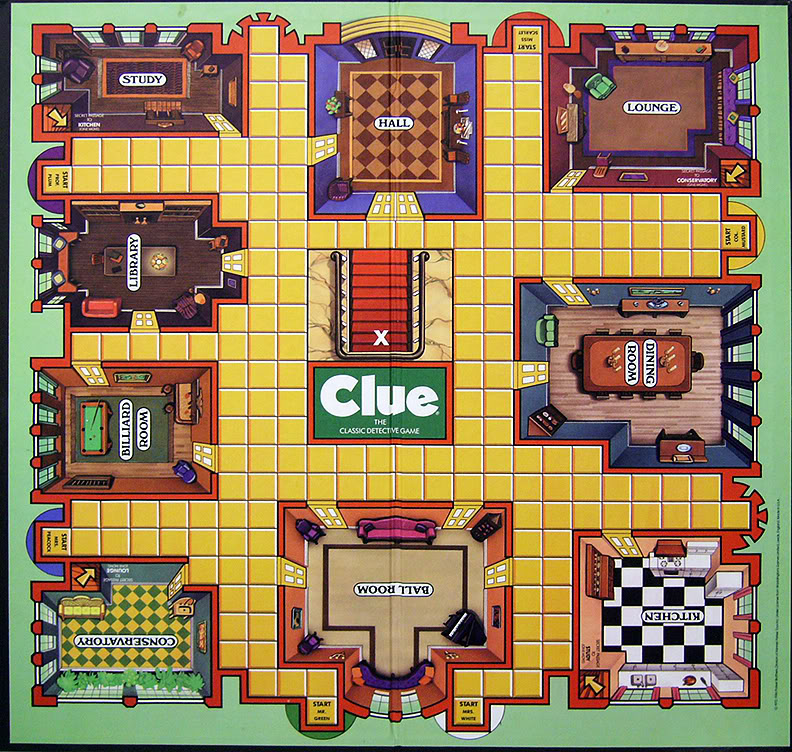
\includegraphics[width=0.5\textwidth]{board.jpg}
	\caption{The game board.}
	\label{fig:board}
\end{figure}

The following principles were observed in this implementation to make it simple:
\begin{itemize}
    \item no long-term planning -- for each action and information received, the agent updates its 'knowledge base' and, on each turn, it makes an independent decision based on the current knowledge, instead of following a planned route;
    
    \item no lucky guesses -- the agent only makes an accusation if it's certain that it's true;
    
    \item no poker face -- the agent only acts to acquire more information, and will not make a move or guess for the sole purpose of misleading other players;
    
    \item no mind reading -- the agent will not infer information from other players actions, except facts that can be logically proven; it will not try to predict how people would or should behave, however, it will assume that everyone will play strategically, \textit{e.g.}, if the player to the left has already shown a certain card before, that card will not be used on a next guess, because a smart player would keep showing the same card over and over again, even if she had a different one to show.
\end{itemize}

The sections below describe the rationale and the details of this implementation. Section \ref{sec:board} explains how the game board and the current position of each player is stored internally and how the agent finds the shortest path to a given goal. Section \ref{sec:data} describes how the knowledge acquired as the match progresses is represented, and how the game decides which action to take on each turn. Finally, Section \ref{sec:interface} brings the predicates that allow the final user to start a new game and interact with the agent.

\section{Moving on the Board}
\label{sec:board}

The game board is seen internally as a grid of size $24\times25$. As illustrated by Figure \ref{fig:board-grid}, coordinates are relative to the lower left corner, and start on $0$.

\begin{figure}[H]
	\centering
	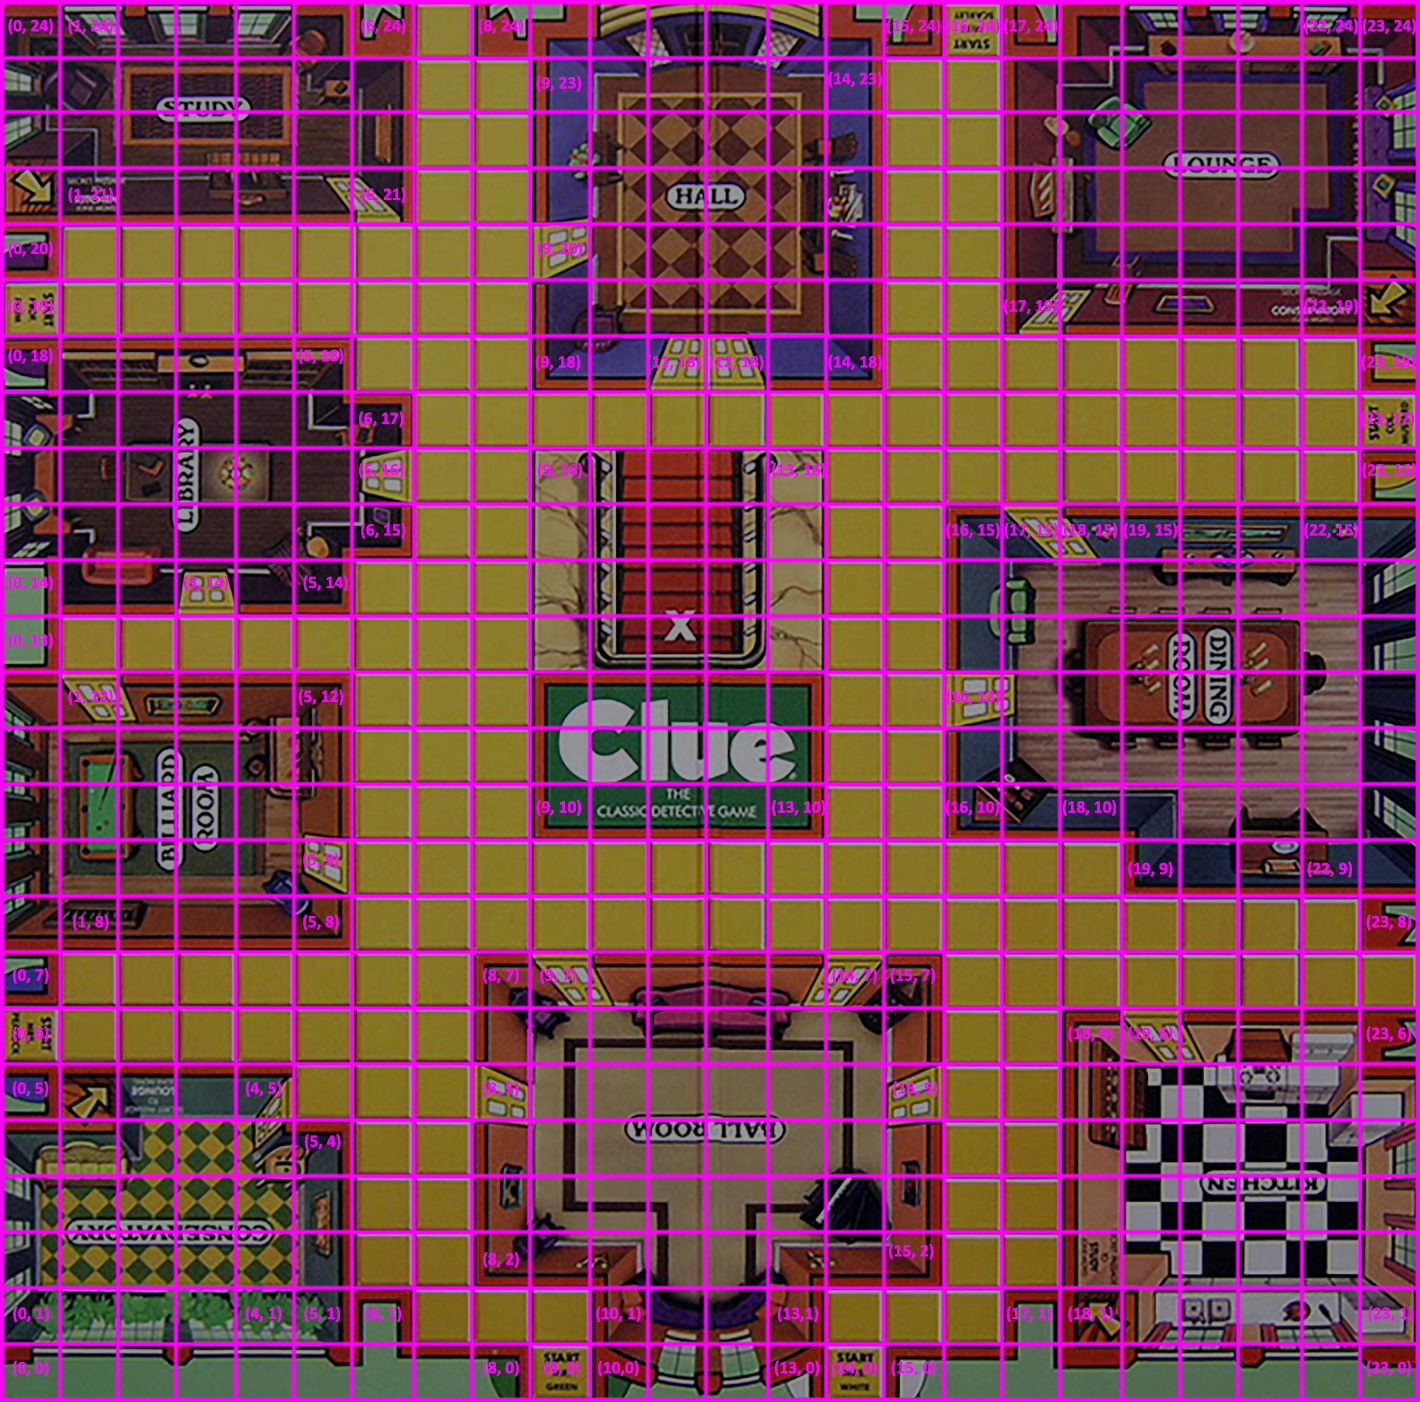
\includegraphics[width=0.95\textwidth]{board-grid.png}
	\caption{The game board.}
	\label{fig:board-grid}
\end{figure}

\subsection{Restrictions}

The following predicates describe the restrictions that affect movements inside the board:
\begin{itemize}
    \item \predprot{blocked}{1} -- is true for the tuple \varname{(X, Y)} if it represents a location that is blocked, \textit{i.e.}, it's inside a room or in a wall;
    
    \item \predprot{door}{2} -- is true for the tuple \varname{(X, Y)} and room \varname{R} if it's possible to enter R from \varname{(X, Y)};
    
    \item \predprot{passage}{2} -- is true for arguments \varname{Source}, \varname{Dest} if there is a secret passage from room \varname{Source} to room \varname{Dest};
    
    \item \predprot{position}{2} (\textit{dynamic}) -- is true for the tuple \varname{(X, Y)} and character \varname{C} if \varname{(X, Y)} is the current position of \varname{C} on the board;
\end{itemize}

Based on the game rules, once inside the room, the position of the individual cell occupied by the player is irrelevant, it's as if each room is a ``supercell''. For that reason, it's only necessary to know if the player is inside a room and, if not, in which (free) cell she is. Also, because each room is accessible only from specific cells, and each of these cells gives access to one, and only one room, it's unnecessary to know if a given cell belongs to a specific room or wall, it's only important to know which are the access cells (\textit{i.e.}, doors) to which room, and if a given cell is free or not.

Since the blocked areas are more ``regular'', \textit{i.e.}, they are more easily described in terms of rectangles, it was a design choice to use a predicate \predname{blocked} that defines if a certain position is blocked or not. The same end could be achieved with an opposite predicate \predname{free}. Figure \ref{fig:blocked} shows the (static) declaration of the blocked cells in the board.

The predicate \predname{door} says if a cell is an access cell, and to which room it gives access to. Since entering the room doesn't count as a step, it's enough to reach these access cells when finding a path and then switching the state to ``inside the room''. Figure \ref{fig:door} shows the (static) declaration of all the doors in the game.

The predicate \predname{passage} is a special case, to represent the information that there are secret passages between the rooms in the (opposite) corners of the board. As shown in Figure \ref{fig:passage}, it is implemented as a commutative operation by using an auxiliary predicate.

Finally, the predicate \predname{position} informs the current position of a player. For any atom \varname{n} that is a valid player name, there will be exactly one fact that says ``the position of \varname{n} is \varname{(X, Y)}''. The agent makes sure this holds true by defining the start position shown on the board once (Figure \ref{fig:start-positions}), and \textit{retracting} and \textit{asserting} that position any time a player's position changes, as will be explained on Section \ref{sec:data}. When a player enters a room, her position becomes that room's name.

Other restrictions, such as the board boundaries, are checked on the path finding algorithm, as described on the next section.

\begin{figure}[hb]
	\centering
\begin{lstlisting}[style=Prolog-pygsty]
%% blocked((X, Y)) - point <X, Y> is inside a room or is a wall
% conservatory
blocked((X, Y)) :- Y =:= 0, X >= 0, X =< 8.
blocked((X, Y)) :- X >= 0, X =< 4, Y >= 1, Y =< 5.
blocked((X, Y)) :- X =:= 5, Y >= 1, Y =< 4.
blocked((6, 1)).
% ball room
blocked((X, Y)) :- X >= 10, X =< 13, Y >= 0, Y =< 1.
blocked((X, Y)) :- X >= 8, X =< 15, Y >= 2, Y =< 7.
% kitchen
blocked((X, Y)) :- Y =:= 0, X >= 15, X =< 23.
blocked((17, 1)).
blocked((X, Y)) :- X >= 18, X =< 23, Y >= 1, Y =< 6.
% dining room
blocked((X, Y)) :- X >= 16, X =< 18, Y >= 10, Y =< 15.
blocked((X, Y)) :- X >= 19, X =< 22, Y >= 9, Y =< 15.
blocked((X, Y)) :- X =:= 23, Y >= 8, Y =< 16.
% lounge
blocked((X, Y)) :- X >= 17, X =< 22, Y >= 19, Y =< 24.
blocked((X, Y)) :- X =:= 23, Y >= 18, Y =< 24.
% hall
blocked((X, Y)) :- X >= 9, X =< 14, Y >= 18, Y =< 23.
blocked((X, Y)) :- Y =:= 24, X >= 8, X =< 15.
% study
blocked((X, Y)) :- X =:= 0, Y >= 20, Y =< 24.
blocked((X, Y)) :- X >= 1, X =< 6, Y >= 21, Y =< 24.
% library
blocked((X, Y)) :- X >= 0, X =< 5, Y >= 14, Y =< 18.
blocked((X, Y)) :- X =:= 6, Y >= 15, Y =< 17.
% billiard room
blocked((X, Y)) :- X =:= 0, Y >= 7, Y =< 13.
blocked((X, Y)) :- X >= 1, X =< 5, Y >= 8, Y =< 12.
% stairs
blocked((X, Y)) :- X >= 9, X =< 13, Y >= 10, Y =< 16.
\end{lstlisting}
	\caption{The declaration of the predicate \predname{blocked}.} 
	\label{fig:blocked}
\end{figure}

\begin{figure}[hb]
	\centering
\begin{lstlisting}[style=Prolog-pygsty]
%% door((X, Y), R) - there's a door to room R from point <X, Y>
door((5, 5), 'conservatory').
door((7, 5), 'ball room').
door((16, 5), 'ball room').
door((9, 8), 'ball room').
door((14, 8), 'ball room').
door((19, 7), 'kitchen').
door((15, 12), 'dining room').
door((17, 16), 'dining room').
door((17, 18), 'lounge').
door((8, 20), 'hall').
door((11, 17), 'hall').
door((12, 17), 'hall').
door((6, 20), 'study').
door((3, 13), 'library').
door((7, 16), 'library').
door((1, 13), 'billiard room').
door((6, 9), 'billiard room').
\end{lstlisting}
	\caption{The declaration of the predicate \predname{door}.} 
	\label{fig:door}
\end{figure}

\begin{figure}[hb]
	\centering
\begin{lstlisting}[style=Prolog-pygsty]
%% passage(Src, Dst) - there's a passage from Src to Dst
passage_aux('conservatory', 'lounge').
passage_aux('kitchen', 'study').
passage(Src, Dst) :- passage_aux(Src, Dst) ; passage_aux(Dst, Src).
\end{lstlisting}
	\caption{The declaration of the predicate \predname{passage}.} 
	\label{fig:passage}
\end{figure}

\begin{figure}[hb]
	\centering
\begin{lstlisting}[style=Prolog-pygsty]
%% position((X, Y), C) - the current position of character C is <X, Y>
%% here, it's initialized to the start position at the board.
%% this predicate will be "rewritten" whenever the script's own
%% character moves or it receives information that another character
%% moved.
:- dynamic position/2.
position((16, 24), 'scarlet').
position((23, 17), 'mustard').
position((14, 0), 'white').
position((9, 0), 'green').
position((0, 6), 'peacock').
position((0, 19), 'plum').
\end{lstlisting}
	\caption{The declaration of the predicate \predname{position} and the initial position of all players.} 
	\label{fig:start-positions}
\end{figure}

\subsection{Path Finding}

One of the key actions the agent must perform is movement. The first step necessary to move on the board is to answer the question: ``where can I go from my current position?''. If the player is in a cell adjacent to a door, she can enter the room; if she is in a corner room, she could use a secret passage. However, to get to the point where she could enter a room, the player must first reach a door, and using a secret passage is a trivial action. Thus, right now, only the problem of moving from a free cell to another free cell will be addressed. In order to solve that problem, the agent must determine the shortest path between two points.

As the game rules state, if the player is currently in any given cell, she can only move to another empty cell vertically or horizontally. To express that relationship, the predicate \predprot{neighbor}{2} is defined (Figure \ref{fig:neighbor}). It will be true for points \varname{(Xs, Ys)}, \varname{(Xn, Yn)} if \varname{(Xn, Yn)} is exactly one cell away from \varname{(Xs, Ys)}, moving either vertically or horizontally (but not both).

\begin{figure}[H]
	\centering
\begin{lstlisting}[style=Prolog-pygsty]
%% neighbor((Xs, Ys), (Xn, Yn)) - <Xn, Yn> is neighbor of <Xs, Ys>.
neighbor((Xs, Ys), (Right, Ys)) :- Right is Xs + 1.
neighbor((Xs, Ys), (Left, Ys)) :- Left is Xs - 1.
neighbor((Xs, Ys), (Xs, Up)) :- Up is Ys + 1.
neighbor((Xs, Ys), (Xs, Down)) :- Down is Ys - 1.
\end{lstlisting}
	\caption{The declaration of the predicate \predname{neighbor}.} 
	\label{fig:neighbor}
\end{figure}

Now, besides checking if a certain cell is a neighbor, it must also be possible to actually move there, \textit{i.e.}, it must be inside the boundaries of the board and not occupied by any other player or blocked, as previously defined. All theses cases are summarized by the predicate \predprot{is\_free}{1}, shown in Figure \ref{fig:is-free}.

\begin{figure}[H]
	\centering
\begin{lstlisting}[style=Prolog-pygsty]
%% is_free((X, Y)) - the position <X, Y> can bee occupied by a character.
is_free((X, Y)) :-
		X >= 0, X =< 23, Y >= 0, Y =< 24, % inside the board
		\+ position((X, Y), _), % not currently occupied by anyone
		\+ blocked((X, Y)). % not a room or a wall
\end{lstlisting}
	\caption{The declaration of the predicate \predname{is\_free}.} 
	\label{fig:is-free}
\end{figure}

Once all the restrictions on movement between two adjacent cells have been represented, it's possible to implement the algorithm to find the shortest path between two points on the map, if such a path exists. More precisely, the algorithm here implemented finds the shortest path between a given free cell \varname{(Xs, Ys)} and the closest door. Subsequent backtracking on the predicate will return all the doors of the board, ascendingly ordered by path length.

The simplest way to tackle this task is using BFS (Breadth-first Search). The idea is simple: inspect the source node; then all the nodes exactly 1 step away from the source node; then all the nodes exactly 2 steps away from the source node; and so on. This ensures that, if a path exists, it will be found and will be a shortest path. If the backtracking mechanism continues from the state where it found a path, the next door found will have the next shortest path.

To make sure that the nodes are inspected in the correct order, a queue is used. This queue begins with the source node. At each iteration, the node at the head of the queue is removed and inspected. If it's not a door, then its adjacent nodes are enqueued and the search continues. To prevent the search from recursing infinitely, it's necessary to keep a set of all nodes seen so far, so only adjacent nodes not yet inspected are enqueued.

The code for this search algorithm is shown in Figure \ref{fig:bfs}. The predicate \predprot{closest\_door}{3} receives a source point and unifies the name of the room with the closest door and the path to that door as a list of points. This predicate itself only sets up the initial values for the algorithm -- the queue and the ``seen nodes'' set are both initialized to a unitary list containing the source point -- and calls the auxiliary predicate \predprot{closets\_door\_aux}{4} to actually perform the search.

The base case for this predicate is when the head of the queue is a door. If that happens, it will unify to the found door's room and the path is a unitary list containing just the door. The recursive step will extract the head of the queue, enqueue all adjacent cells that are free and have not yet been seen (described by \predprot{valid\_adjacent}{3}), mark all the neighbor cells are seen, and recursively continue walking on the list. As the recursive calls return, the path is built by inserting the inspected node on the head of the result list.

\begin{figure}[H]
	\centering
\begin{lstlisting}[style=Prolog-pygsty]
%% closest_door((Xs, Ys), Room, Path) - starting at <Xs, Ys>, finds
%% the closest Room door and the Path to it
valid_adjacent((X, Y), (Xd, Yd), Seen) :-
		neighbor((X, Y), (Xd, Yd)),
		\+ member((Xd, Yd), Seen),
		is_free((Xd, Yd)).
closest_door_aux(Room, [(X, Y)], [(X, Y)|_], _) :- door((X, Y), Room).
closest_door_aux(Room, [(X, Y)|PTail], [(X, Y)|QTail], Seen) :-
		% enqueues all non-seen adjacents to which it's possible to move
		findall((Xd, Yd), valid_adjacent((X, Y), (Xd, Yd), Seen), ValidAdjacents),
		append(QTail, ValidAdjacents, Queue),
		% stores all adjacent nodes as seen, to cut the search recursion
		findall((Xa, Ya), neighbor((X, Y), (Xa, Ya)), Neighbors),
		union(Neighbors, Seen, NewSeen),
		closest_door_aux(Room, PTail, Queue, NewSeen). % recursive definition
closest_door((Xs, Ys), Room, Path) :-
		is_free((Xs, Ys)),
		closest_door_aux(Room, Path, [(Xs, Ys)], [(Xs, Ys)]).
\end{lstlisting}
	\caption{The breadth-first search used to navigate on the map.} 
	\label{fig:bfs}
\end{figure}

\section{Representing Knowledge}
\label{sec:data}

\section{The Interface}
\label{sec:interface}

\end{document}
